\documentclass{article}
\usepackage[hidelinks]{hyperref}
\usepackage{tikz}


\begin{document}
\begingroup
\centering
\LARGE AIS Testrapport Futronic \\
\endgroup
\section{Skriv ned info}
\subparagraph{Skipstype}
\subparagraph{AIS-type}
\subparagraph{Serienummer}
\section{Klargj\o{}r Futronic}
\subsection{Slett gammel data}
Test Reports$\rightarrow$Clear Memory
\subsection{Legg inn b\aa{}tens MMSI}
Edit ship's MMSI
\section{Utf\o{}r tester}
\subsection{Request Message 5 AIS1}
\subsubsection{Kobling}
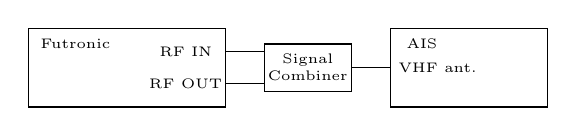
\begin{tikzpicture}%message 5
\draw (0,0) -- (2.5,0) -- (2.5,1) -- (0,1) -- (0,0);
\node at (.6,.8){\tiny{Futronic}};
\node at (2.0,.7){\tiny{RF IN}};
\node at (2.0,.3){\tiny{RF OUT}};
\draw (2.5,.7) -- (3,.7);
\draw (2.5,.3) -- (3,.3);
\draw (3,.2) -- (4.1,.2) -- (4.1,.8) -- (3,.8) -- (3,.2);
\node at (3.55,.6){\tiny{Signal}};
\node at (3.55,.4){\tiny{Combiner}};
\draw (4.1,.5) -- (4.6,.5);
\draw (4.6,0) -- (6.6,0) -- (6.6,1) -- (4.6,1) -- (4.6,0);
\node at (5.2,.5){\tiny{VHF ant.}};
\node at (5.0,.8){\tiny{AIS}};
\end{tikzpicture}
\\
\subsubsection{AIS1}
AIS tests$\rightarrow$Set no.: 1$\rightarrow$Request MSG 5$\rightarrow$AIS1 161.975 Mhz
\clearpage
\subsection{Receive AIS sele}
\subsubsection{Kobling}
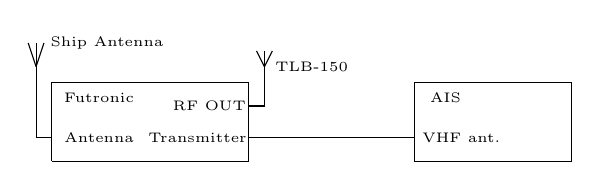
\begin{tikzpicture}%Receive AIS sele
\draw (0,0) -- (2.5,0) -- (2.5,1) -- (0,1) -- (0,0);
\node at (.6,.8){\tiny{Futronic}};
\node at (2.0,.7){\tiny{RF OUT}};
\draw (2.5,.7) -- (2.7,.7) -- (2.7,1.2);
\draw (2.7,1.2) -- (2.6, 1.4);
\draw (2.7,1.2) -- (2.7, 1.4);
\draw (2.7,1.2) -- (2.8, 1.4);
\node at (3.3,1.2){\tiny{TLB-150}};
\node at (1.85,.3){\tiny{Transmitter}};
\draw (2.5,.3) -- (4.6,.3);
\node at (.6,.3){\tiny{Antenna}};
\draw (0,.3) -- (-.2,.3) -- (-.2,1.2);
\draw (-.2,1.2) -- (-.3, 1.5);
\draw (-.2,1.2) -- (-.2, 1.5);
\draw (-.2,1.2) -- (-.1, 1.5);
\node at (.7,1.5){\tiny{Ship Antenna}};
\draw (4.6,0) -- (6.6,0) -- (6.6,1) -- (4.6,1) -- (4.6,0);
\node at (5.2,.3){\tiny{VHF ant.}};
\node at (5.0,.8){\tiny{AIS}};
\end{tikzpicture}
\subsubsection{AIS1}
AIS tests$\rightarrow$Set no.: 1$\rightarrow$Receive AIS sele$\rightarrow$AIS1 161.975 Mhz 
\subsubsection{AIS2}
AIS tests$\rightarrow$Set no.: 1$\rightarrow$Receive AIS sele$\rightarrow$AIS2 162.025 Mhz
\section{Generer rapport}
\subsection{Last ut loggfil}
Koble Futronic-en til pc-en med den vedlagte USB-kabelen. \\
\AA{}pne programmet FUTRONIC test box MKII og lagre loggfilen. \\
Programmet kan lastes ned her \href{http://www.danphone.com/Default.aspx?ID=48}{\underline{http://www.danphone.com/Default.aspx?ID=48}} 
\subsection{Lag installasjonrapport}
\AA{}pne rapportprogrammet \\
Velg loggfil\\
Fyll inn skipstype, AIS-type og serienummer \\
Trykk "Lag Rapport" \\
Programmet kan lastes ned her \href{https://github.com/eier7/futronic}{\underline{https://github.com/eier7/futronic}} 


\end{document}
